%\documentclass[twoside]{pwrthesis}
\documentclass[twoside]{iisthesis}
% ---
\usepackage[utf8]{inputenc}
\usepackage[T1]{fontenc}
\usepackage[polish]{babel}
\usepackage{graphicx}
\usepackage{amsmath}
\usepackage{listings}
\usepackage{algorithmic}
\usepackage{algorithm}
\usepackage{subfig}

% Dodane przeze mnie d
\usepackage{fancyvrb} % dla srodowiska Verbatim
\usepackage{color}
\usepackage{lscape}


% definicje kolorow
\definecolor{ciemnoSzary}{rgb}{0.15,0.15,0.15}
\definecolor{szary}{rgb}{0.5,0.5,0.5}
\definecolor{jasnoSzary}{rgb}{0.2,0.2,0.2}

% Konfiguracja verbatima
\fvset{
	frame=single,
	numbers=left,
	fontsize=\footnotesize,
	numbersep=12pt,
%	framerule=.5mm,
	rulecolor=\color{ciemnoSzary},
%	fillcolor=\color{jasnoSzary},
	framesep=4pt,
	stepnumber=1,
	numberblanklines=false,
	tabsize=2,
%	formatcom=\color{szary}
}

\begin{document}

\title{Rozpoznawanie obrazów podobnych przy użyciu podejścia wzorowanego na korze wzrokowej.}
\author{Adam Puchalski}
\advisor{dr hab. inż. Urszula Markowska-Kaczmar}
\instituteLogo{logos/pwr}
\slowaKluczowe{kora wzrokowa\\rozpoznawanie obrazów\\sztuczna inteligencja}

\date{\number\the\year}

% Wstawienie abstractu pracy
	%\input {abstract}
	
\abstractSH{
Praca obejmuje opis kilku podejść -- w tym jedno autora -- w rozpoznawaniu obrazów, które bazują na korze wzrokowej ssaków. }

\abstractPL{
%TODO
	Abstrakt
}
\abstractEN{
%TODO
	Abstract
}

\maketitle
\textpages


\chapter*{Wprowadzenie}
Rozpoznawanie obrazów jest jednym z najważniejszych zastosowań sztucznej inteligencji. Właściwie, aby można było mówić o sztucznej inteligencji konieczne jest uwzględnienie zaawansowanych technik rozpoznawania obrazów. Mimo, że zdecydowana większość problemów sztucznej inteligencji jest problemami trudnymi\footnote{W literaturze angielskojęzycznej określa się to pojęciem AI-complete.}, to wydaje się, że na równi z rozpoznawaniem języka, jako podstawowe należy uznawać rozpoznawanie obrazów.\\

W tej pracy przedstawione będą podstawowe techniki stosowane w rozpoznawaniu obrazów, które w idei mają być komputerowym odpowiednikiem kory wzrokowej. Techniki te są mniej lub bardziej związane z dziedzinami rozpoznawania obrazów w grafice komputerowej i naukami o mózgu, które wcześniej wspomnianej kory wzrokowej dotyczą. Można by pokusić się o narysowanie odcinka na płaszczyźnie, którego końcami byłby te dwie dziedziny. Wtedy wszystkie istniejące projekty dotyczące rozpoznawania obrazów można by umieścić na tej płaszczyźnie. Były by one umiejscowione na tym odcinku w pewnej odległości, która określałaby powiązanie z konkretną dziedziną. Celem tej pracy jest znalezienie tego najlepszego punktu na tym odcinku, który będzie wykorzystywać zaawansowane techniki z dziedziny rozpoznawania obrazów i te zaobserwowane w korze wzrokowej. Zagadnienie to zostało sprowadzone do jednego wymiaru celowo, żeby pokazać skąd należy czerpać inspiracje, faktem jest jednak, że ciężko jest wyrazić złożoność tematu w jednym wymiarze. Aby lepiej przedstawić to co się dzieje w dziedzinie należałoby zdaniem autora skupić się na korze wzrokowej i dzieląc ją na elementy pokazać co, gdzie i w jaki sposób jest przedstawiane.



\chapter{Biologiczne podstawy pracy}
%TODO S pending!
\section{Mózg człowieka}
\label{mozg}
%
% strona 493
% strona 469
%
Przy opisie mózgu człowieka wypada zacytować pewne porównanie, na jakie pokusił się David H. Hubel w swoim artykule z kwietnia 1978 roku \cite{Hubel1978}. Przedstawia on powody, przez które jest trudno mózg badać. Przede wszystkim skomplikowanie wiążące się z liczbą komórek z których się składa -- $10^{10}$, chociaż w tamtych czasach mówiło się nawet o $10^{11}$. Dzisiaj mówi się o liczbie $2 \cdot 10^{10}$ \cite{encyclopedia} lub (w tej samej encyklopedii) $11-12 \cdot 10^{9}$. Wracając jednak do Hubela, liczba komórek w mózgu to nie jedyna bariera. Przywołuje on jako przykład wątrobę, która składa się jedynie z dwóch różnych komórek, które pracując wspólnie wykonując około 15 różnych funkcji, zakładając, że ich liczba może być większa. W mózgu natomiast szacuje się, że istnieje od $100$ do $500$ różnych komórek -- w zależności od dokładności z jaką zostaną podzielone. Hubel nie zaryzykował szacowania liczby różnych funkcji mózgu. Wspomniał jednak, że dodatkowe skomplikowanie jest powodowane przez połączenia komórek ze sobą, które -- jak można przypuszczać -- przypominają gęstą sieć. W cytowanej wyżej encyklopedii, która jest podstawą kolejnych części tej pracy, szacuje się, że każda komórka jest powiązana z około $10^4$ innych co powoduje, że całkowita liczba połączeń synaptycznych może przekroczyć całkowitą liczbę cząsteczek występujących na ziemi. Przez co cały czas ludzki mózg jest dla naukowców zagadką i zarówno w 1978 roku jak i teraz więcej jest pytań jego dotyczących niż odpowiedzi.

\section{Wydzielone obszary w mózgu}
\label{obszaryWMozgu}
Mózg człowieka, mimo, że nie od samego początku uważany za organ odpowiadający za myślenie i przetwarzanie wszelkich informacji z otaczającego środowiska, był dla naukowców zawsze zagadką. To co dzisiaj wiadomo o mózgu jest efektem prac tysięcy naukowców, którzy podzielili mózg na dziesiątki obszarów. Pierwszy taki podział był zaproponowany w 1907 roku przez Korbiniana Brodmana. Podzielił on mózg na 47 obszarów \cite{brodmannn} ze względu na różnice w strukturze warstwowej i komórkowej. Kora wzrokowa -- podzielona na pierwotną (pierwszorzędową), drugorzędową oraz trzeciorzędową -- miała numery odpowiednio 17, 18 i 19. Dodatkowo utrwaliło się w literaturze oznaczenie V1, V2 i V3, które odnosi się tylko do tych obszarów i również odpowiada polom 17, 18 i 19.

\section{Kora wzrokowa}
\label{badaniaKoryWzrokowej}
Zanim zostanie przybliżona struktura kory wzrokowej należy wspomnieć o tym w jaki sposób wiedza, którą posiadamy na temat tej części mózgu jest poszerzana. Niektóre badania prowadzone są z udziałem ludzi posiadających najogólniej uszkodzenia kory wzrokowej \cite{Girkin2001}. Do tych patologii należą:
\begin{itemize} 
\item ślepota -- ta, która nie jest wynikiem wad wrodzonych oka, bądź innych, tylko jest spowodowana uszkodzeniami natury neurologicznej (czytając tekst napisany językiem Braille\'a aktywowane są obszary kory wzrokowej)
\item achromatopsia -- agnozja barw) -- niezdolność do rozpoznawania barw nawet jeśli oko jest zdolne do ich rozpoznawania
\item akinetopsja -- powszechnie nazywana ślepotą ruchu %------%http://en.wikipedia.org/wiki/Akinetopsia
\item prosopagnozja -- ślepota twarzy \cite{Gauthier1999}
%TODO dodać więcej
\end{itemize}

Mając takiego osobnika można doszukiwać się szczegółów dotyczących jego niepełnosprawności, a co za tym idzie przyczyn, skutków, miejsca w którym się znajduje i innych. Wydobywając informacje o wielu patologiach z wielu przypadków dosyć prosto jest je uogólnić i dojść do wniosku, że nie tylko ludzie, ale i wszystkie ssaki mogą mieć podobną strukturę i działanie. Mając takie informacje badania można prowadzić na zwierzętach (myszach, kotach, małpach) co dalej rozwija tą naukę. Należy się jednak szczególna uwaga w kwestii interpretacji wyników badań mózgów małp, na co zwraca uwagę autor pracy \cite{Kaas1995}.\\

Nie tylko z patologii kory wzrokowej można uzyskiwać informacje o tej części mózgu. Jeden z przykładów prezentowanych w encyklopedii \cite{encyclopedia} pokazuje kota z założoną do kory wzrokowej elektrodą. Jest ona przyłączona do oscyloskopu, aby w ten sposób wizualizowane wyniki przedstawiały impulsy, które są w danej części mózgu kory przesyłane. Dzięki temu zabiegowi możliwe jest badanie aktywności kory wzrokowej względem obrazów, jakie są kotu przedstawiane.\\

Wymieniona wcześniej prosopagnozja jest chorobą neurologiczną, której skutkiem -- u osoby chorującej -- jest niemożność rozpoznawania twarzy. Wykrycie takiego zaburzenia u człowieka spowodowało powstanie teorii, że istnieje specjalna część kory wzrokowej, która odpowiada za rozpoznawanie twarzy w mózgu \cite{Gauthier1999}. Posługując się techniką funkcjonalnego magnetycznego rezonansu jądrowego można stwierdzić nawet wiele więcej. Autorzy pracy \cite{Downing2001} twierdzą, że w mózgu są specjalne struktury, odpowiedzialne za rozpoznawanie ludzkiego ciała. Idąc tym tropem, autor pracy \cite{Grill-Spector2003} badał obszary w korze wzrokowej, które uaktywniają się podczas pokazania badanemu pacjentowi różnych zdjęć. Na tej podstawie był w stanie określić miejsca aktywujące się na widok miejsc, obiektów, bądź twarzy. Okazało się też, że odnalezione w ten sposób obszary wykazują większą aktywność, jeśli zdjęcie przedstawia coś znanego niż coś, czego badany nie znał.\\
%\Citeauthor{Grill-Spector2005}
Cytowany wcześniej Grill-Spector badając ludzką korę wzrokową i jej reakcje na przedstawiane obrazy doszedł do kolejnych ciekawych wniosków. Okazuje się, że przy pokazywaniu obrazów człowiekowi, tak samo szybko jest on w stanie stwierdzić, czy na obrazie jest jakiś obiekt (detekcja) jak i to, do jakiej klasy on należy (kategoryzacja) \cite{Grill-Spector2005}. Identyfikacja obiektu zawsze wymagała więcej czasu.\\

W ramach ciekawostki można też wspomnieć o obszarach w mózgu, które są wrażliwe na ruch obrotowy \cite{kahana2010}. O co chodzi w tym określeniu najlepiej tłumaczy sposób, w jaki autorzy tej pracy do takiego wniosku doszli. Badali oni aktywność pewnych obszarów mózgu podczas jazdy po rondzie raz zgodnie, a innym razem przeciwnie do ruchu wskazówek zegara. 

\section{O wzroku słów kilka}
\label{oWzrokuSlowKilka}
Nie sposób opisać biologicznych podstaw rozpoznawania obrazów u człowieka nie zaczynając od oka, a przecież ono jest najbardziej namacalnym i pierwszym za razem elementem toru, którym informacja wizualna jest przekazywana do mózgu.\\

Oko wprawdzie nie spełnia specjalnie skomplikowanego zadania. Twierdzi się nawet, że oko jest elementem czysto mechanicznym, który odpowiednio przygotowuje wiązkę światła do momentu, w którym pada ono na siatkówkę. Na niej wyświetlany jest obraz widziany przez oko, jest on znacznie pomniejszony i obrócony. Siatkówka jest pewnego rodzaju błoną, wyposażoną w fotoreceptory. W nich następuje zmiana sygnału wizualnego na sygnał chemiczny. Informacja wizualna w postaci chemicznej jest przekazywana nerwem wzrokowym do ciała kolankowatego bocznego, a stamtąd przenoszona do pierwotnej kory wzrokowej.

\section{Struktura kory wzrokowej}
\label{strukturaKoryWzrokowej}
%
% 673 dobre!
%
Kora wzrokowa jest podzielona na obszary, które pełnią różne funkcje. Przedstawiają one jakby kolejne etapy przetwarzania bodźców wizualnych, jednak istnieją odstępstwa od tej reguły w postaci połączeń między-warstwowych. Mimo, że cały czas prowadzone są debaty co do zarówno liczby jak i granic wydzielanych obszarów w korze wzrokowej \cite{Kaas1995}, naukowcy są zgodni co do wielości i zróżnicowania obszarów występujących w płacie potylicznym, w którym znajduje się kora wzrokowa. Prowadzone badania w tym zakresie są również zgodne co do początku neurologicznej części szlaku wzrokowego, którym jest pierwszorzędowa kora wzrokowa.

\label{v1}
\subsection{Pierwszorzędowa kora wzrokowa -- V1}
Inaczej nazywana pierwotną korą wzrokową, lub obszarem V1, odpowiada jej również numer 17 Brodmanna. Najważniejszych informacji dotyczących tej części kory wzrokowej dały prace Davida H. Hubela oraz Torstena N. Wiesela, które zostały w roku 1981 nagrodzone nagrodami Nobla w dziedzinie medycyny \cite{hubelnobel,wieselnobel}.\\

\begin{figure}[ht]
	\centering
	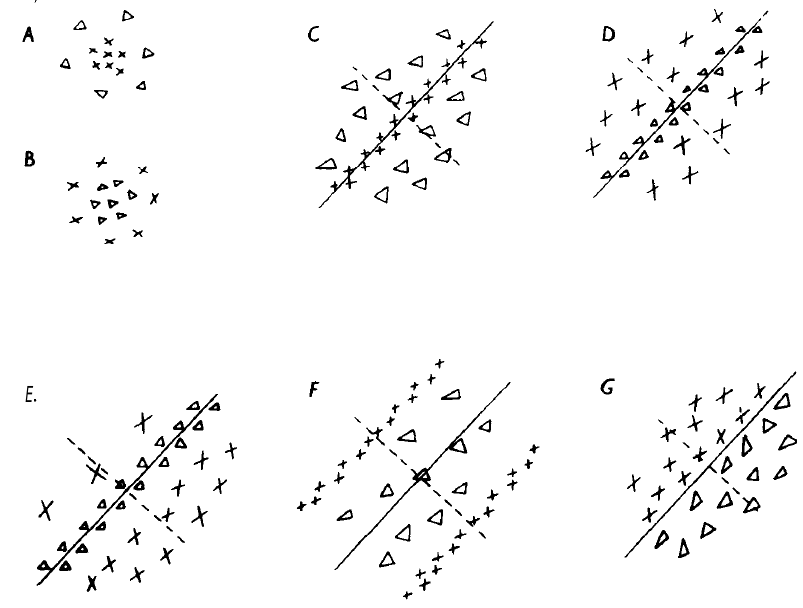
\includegraphics[width=1.00\textwidth]{images/HandW.png}
	\caption{Punkty A i B przedstawiają pola wzbudzeń, neuronów z ciała kolankowatego bocznego, co również odpowiada komórkom siatkówki oka. Punkty C-G przedstawiają pola wzbudzeń neuronów pierwotnej kory wzrokowej, które są wrażliwe na istniejące w obrazie kreski, bądź krawędzie pod określonym kątem, lecz różnych rozmiarów. Można sobie wyobrazić, że w korze wzrokowej dla bardzo wielu nachyleń kąta są podobne grupy neuronów \cite{hubelnobel}.}
	\label{fig:handw}
\end{figure}

Podstawowym faktem, jaki zaobserwowali naukowcy był fakt istnienia neuronów, których aktywność ściśle zależna jest od określonego obszaru na siatkówce (receptive field -- RF). W ten sposób można by określić pole na siatkówce, którego wyjście stanowi wzbudzenie dla tego neuronu. Podobnie więc jak na siatkówce każdy fotoreceptor odpowiada za fragment obrazu, tak w pierwotnej korze wzrokowej każdemu fragmentowi obrazu odpowiada pewna grupa neuronów. Dodatkowo badając wzbudzenie tych neuronów odkryli, że konkretne obszary pierwotnej kory wzrokowej są czułe na występujące w obrazie (odwzorowane na siatkówce) kreski (jasne i ciemne -- rysunek \ref{fig:handw} C-F) lub wyraźne krawędzie (rysunek \ref{fig:handw} G) będące w jego polu. Wzbudzenie neuronu dodatkowo ściśle zależy od kąta pod którym dane kreski się znajdują oraz miejsca, w którym w polu wpływającym na wzbudzenie komórki się znajduje. Naukowcy zdecydowali się nazwać te neurony komórkami złożonymi, najprawdopodobniej z powodu, że na jeden neuron składa się bardzo wiele komórek siatkówki, a przez to również ciała kolankowatego bocznego (których pola wzbudzeń przedstawione są na rysunku \ref{fig:handw} A i B), przez co reprezentuje on pewien kompleks komórek. Co może nie do końca wydawać się oczywiste, każdemu fragmentowi obrazu odpowiada szereg neuronów, których budowa jest taka sama, a różnią się jedynie kątem kreski, na który są szczególnie wrażliwe.\\

Na takiej samej zasadzie określa się istnienie w pierwotnej korze wzrokowej neuronów, wrażliwych na wcześniej wspomniane kreski poruszające się w określonym kierunku jak i istnieniu konkretnego koloru we fragmencie obrazu. Dodatkowo okazało się, że pole wrażliwości neuronów -- komórek złożonych -- ma różne wielkości i pola te się wzajemnie pokrywają. \\

Naukowcy wprowadzili również pojęcie komórek hiper-złożonych, które stanowiły połączenie kilku komórek złożonych. Takie komórki udało się zlokalizować u zwierząt pokazując im kreski określonej długości.\\

Oprócz odkrycia elementów pierwotnej kory wzrokowej, naukowcy umiejscowili je w bardziej złożonych strukturach, które nazywane były kolumnami orientacyjnymi i miały konkretne miejsce w pierwotnej korze wzrokowej w mózgu.

\subsection{Pozostałe warstwy kory wzrokowej}
\label{restOfTheVisualLayers}
Przez cały czas, począwszy od odkryć Davida H. Hubela oraz Torstena N. Wiesela, prowadzone są badania, mające na celu uszczegółowienie całej kory wzrokowej jak i samego mózgu. Przeglądając osiągnięcia naukowców można stwierdzić, że istnieje ponad 30 różnych obszarów w mózgu, których sposób połączenia nie jest jednak do końca jasny. Przedstawianych jest wiele modeli kory wzrokowej, z których wiele jest szczegółowych, mających na celu reprezentację architektury mózgu -- tego co i jak jest połączone wewnątrz \cite{Ungerleider}. Z perspektywy informatyka można by pokusić się o porównanie szczegółowych modeli mózgu do grafu, którego węzłami są obszary mózgu, a krawędziami połączenia między tymi obszarami. Ciągła praca naukowców na tym polu powoduje, że odnajdywane są nowe sposoby współdziałania obszarów mózgu, przez co graf ten nieuchronnie zmierza do grafu pełnego, potwierdzając tym samym skomplikowanie mózgu. Inne modele natomiast przedstawiają struktury zainspirowane nauką o korze wzrokowej, których celem jest mieć przede wszystkim zastosowanie praktyczne.\\

Nim autor skupi się na zastosowaniach praktycznych -- które są ściśle związane z tematyką pracy -- przedstawiony zostanie główny podział, na dwa strumienie informacji wzrokowej, których początkiem jest pierwszorzędowa kora wzrokowa \cite{Ungerleider}.\\
\begin{description}
\item [Szlak brzuszny] -- ventral stream -- odpowiedzialny za identyfikację widzianych obiektów
\item [Szlak grzbietowy] -- dorsal stream -- odpowiedzialny za relacje między obiektami oraz poruszanie się obiektów w przestrzeni
\end{description}

%TODO szlaki - rysunek

Mimo, że w związanych z dziedziną artykułach nie jest to powiedziane w prost, większość realizacji kory wzrokowej (we wspomnianych zastosowaniach praktycznych) opisuje szlak brzuszny, a więc samą identyfikację widzianych obiektów. Realizacja obu zadań nie jest prosta. Jeszcze trudniejsze jest powiązanie ich ze sobą. Marzeniem wszystkich projektantów kolejnych podejść w tej dziedzinie jest jednak stworzenie takiego systemu, który podobnie jak wzrok człowieka jest w stanie rozpoznawać, kategoryzować, \ldots \ widziane obiekty.\\

Opis pozostałych -- wszystkich z wyłączeniem pierwotnej -- warstw kory wzrokowej można właściwie w tym momencie przerwać. Co było bowiem sygnalizowane wcześniej, naukowcy mają problem z określeniem struktury, pełnionych funkcji, umiejscowienia jak i połączeń ze sobą kolejnych -- wyższych warstw kory wzrokowej.\\

Przedstawione poniżej architektury czerpią w mniejszym, bądź większym stopniu z przedstawianych w literaturze modeli funkcjonowania mózgu. Wspólną ich cechą jest jednak bezsprzecznie pierwotna kora wzrokowa. 


\chapter{Modele kory wzrokowej z zastosowaniem praktycznym}
\label{praktyczneModeleKoryWzrokowej}

Z konstrukcją systemów rozpoznających obrazy, szczególnie tych, bazujących na odkryciach w korze wzrokowej są wciąż trudności. Wiadomo bowiem co się mniej więcej dzieje w głowie, jak informacja wizualna jest przekazywana i każdy może się domyślić jak ma wyglądać efekt rozpoznawania obrazów. W kwestii realizacji -- zgodnie z wstępem do tej pracy -- jest różnie. W każdej publikacji, która opisuje jedno z proponowanych rozwiązań przedstawiony jest punkt widzenia, rzadko opisujący zaawansowany etap przetwarzania obrazu. Najczęściej są to etapy początkowe, przedstawiające transformacje mające miejsce w pierwszorzędowej korze wzrokowej, a więc ekstrakcję i integrację konturów. Nie spotykane są konkretne propozycje rozwiązań problemów występujących w wyższych warstwach kory wzrokowej samodzielnie. Ciężko bowiem jest określić podstawy, bądź jakąś bazę, na której można by budować dalej. Co autorzy rozwiązań podkreślają bardzo często, problematyka jest już na poziomie odzyskiwania krawędzi z obrazów.\\

Wprawdzie ,,kompletne'' modele wykorzystujące elementy kory wzrokowej w rozpoznawaniu obrazów też się pojawiają, nie sposób zacząć jednak inaczej jak właśnie od ekstrakcji i integracji samych konturów.

\section{Ekstrakcja i integracja konturów}
\label{contourIntegration}

%DONE%TO DO - 30k10, 
\subsection{Ekstrakcja konturów z obrazu}
\label{integracjaSEC}

%SEC - 30k10
%http://www.int.washington.edu/talks/WorkShops/int_03_1/People/Schlei_B/INT2003.pdf

Algorytmów na ekstrakcję konturów z obrazu jest bardzo wiele, na dziesiątki różnych sposobów można szukać krawędzi obiektów na nich się znajdujących. Mimo, że jest ich wiele, i wyniki ich działania są zadowalające -- chociaż z entuzjazmem najczęściej wypowiadają się sami autorzy -- to problem jest trochę gdzie indziej. Krawędzie odzyskane z obrazów klasycznymi algorytmami, wciąż są pikslami w obrazie, które wprawdzie dla ludzkiego oka stanowią lepsze lub gorsze odwzorowanie konturów, ale do dalszego przetwarzania muszą być dodatkowo przygotowane. Jest to spowodowane przede wszystkim wymaganiami podyktowanymi przez temat tej pracy, który zakłada czerpanie z kory wzrokowej jako źródła inspiracji dla algorytmów. W związku z czym wymagane jest przetwarzanie otrzymanych obrazów przedstawiających krawędzie do struktur danych reprezentujących te krawędzie.\\

Przedstawiony więc będzie jeden z wielu algorytmów, który z obrazów odzyskuje kontury z obrazu cyfrowego.


\label{diconex}
\subsubsection{DICONEX}

Algorytm -- co podkreślają twórcy -- jest perfekcyjny w sensie wyznaczania krawędzi obiektów jeśli przyjmie się następujące kryteria:
\begin{itemize}
\item obszary się wzajemnie nie przecinają,
\item obszary są niepuste,
\item nie ma ograniczeń na 2 wymiary,
\item szybkość działania
\end{itemize}
Algorytm pracuje na obrazach monochromatycznych, więc wymaga się przekształcenia np. zdjęć do skali szarości.

\begin{figure}[ht]
	\centering
	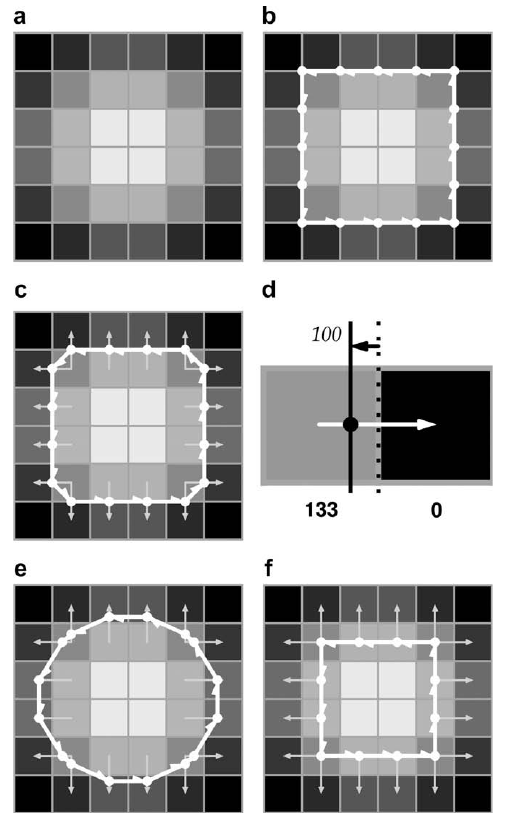
\includegraphics[width=.55\textwidth]{images/DICONEX_EX.png}
	\caption{Przykład działania algorytmu DICONEX na obrazie w skali szarości, o rozmiarach $6 \times 6$ \cite{Schlei2009}.}
	\label{fig:diconex_ex}
\end{figure}

\begin{figure}[ht]
	\centering
	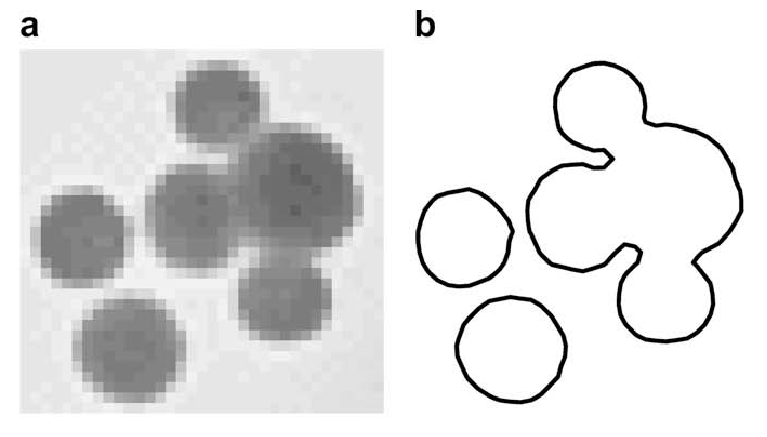
\includegraphics[width=.70\textwidth]{images/DICONEX_EX_RES.png}
	\caption{Wynik (b) działania algorytmu DICONEX na obrazie niewielkiej rozdzielczości (a) \cite{Schlei2009}.}
	\label{fig:diconex_ex_res}
\end{figure}

\label{dixonex_alg}
\subsubsection{Algorytm}

Na początku algorytmu wymagane jest wybranie jednej -- granicznej wartości jasności dla obrazu. W przykładzie z pracy \cite{Schlei2009}, dla obrazu, którego jasność piksli jest z zakresu $0 - 155$ została ona obrana na poziomie 100. Rysunek \ref{fig:diconex_ex}A przedstawia wejściowy obraz. W pierwszym kroku algorytmu, w obrazie wektorami konturowymi (ang. contour vector) otaczane są piksle o wartości jasności większej niż 100 -- czyli jasne piksle -- czego wynik przedstawiany jest na rysunku \ref{fig:diconex_ex}b. Warto zauważyć, że wspomniane wektory konturowe zawsze zwrócone są w taką stronę, że po lewej stronie mają otaczany obiekt -- czyli w tym wypadku piksle o jasności większej niż 100. Zgodnie z tym algorytmem zawsze znalezione wektory będą ze sobą połączone na zasadzie początek jednego wektora z końcem drugiego wektora i nie będzie pustych obszarów. Jako kolejny krok algorytmu, wszystkie stworzone wektory zamieniane są na inne wektory, o tej samej orientacji, ale ich punkty zaczepienia znajdują się w na środku wyznaczonego wcześniej wektora krawędziowego (konturowego), a kończą się w środku kolejnego wektora krawędziowego. Po zastosowaniu się do tego przekształcenia obraz otrzymany powinien wraz z krawędzią wyglądać tak jak na rysunku \ref{fig:diconex_ex}c. Dodatkowo na tym rysunku przedstawione są pewne wektory, które w cytowanej publikacji nazywane są wektorami zakresu (ang. range vector). Wektory te są umieszczone w obrazie w taki sposób, że łączą środki sąsiednich piksli i przechodzą przez każdy środek wektora konturowego a ich zwrot jest skierowany na zewnątrz otaczanego obszaru. Rysunek \ref{fig:diconex_ex}d przedstawia 2 piksle z obrazu, między którymi znajdował się środek wektora konturowego. W kolejnym kroku algorytmu punkt ten będzie przesunięty na wektorze zakresu w taki sposób, że obrana na samym początku wartość jasności (równa 100) będzie znajdować się na tym wektorze, gdy między środkowymi punktami piksli wartość ich jasności będzie liniowo interpolowana. Wynik takiego działania przedstawiony jest na rysunku \ref{fig:diconex_ex}e. Rysunek \ref{fig:diconex_ex}f przedstawia wynik transformacji tego poszerzonego konturu do konturu oznaczającego granicę szukanego obszaru. Jednak jak widać na przykładzie to przekształcenie jakby cofało wszystkie uogólnienia, zaokrąglenia i właściwie same przekształcenia, które zostały znalezione w obrazie \ref{fig:diconex_ex}c i \ref{fig:diconex_ex}e. Zdaniem autora najlepszy rezultat zaprezentowany jest na rysunku \ref{fig:diconex_ex}e.\\

O ile sam algorytm jest ciekawy, to został on tutaj zaprezentowany głównie z powodu na efekty, jakie można uzyskać w innych nietrywialnych obrazach, w a szczególności tych, niewielkich rozmiarów. Rysunek \ref{fig:diconex_ex_res} przedstawia wynik działania algorytmu na obrazie słabej rozdzielczości. Wyraźnie widać, że kontury odtworzone przez algorytm są wyraźne i gładkie, co jest niewątpliwą zaletą.\\

Z zastosowaniem tego algorytmu jest jednak podstawowy problem, który polega na konieczności obrania wartości granicznej dla jasności grup piksli w obrazie. Podobne problemy mają inne algorytmy odnajdujące krawędzie w obrazie. Można by się spierać, który jest lepszy, fakt jest jednak taki, że w oryginalnej postaci wymagają określania dodatkowych specyficznych parametrów.\\

Trochę inaczej można podejść do tego zagadnienia metodami zaczerpniętymi wprost z grafiki komputerowej -- filtrami. Dla obrazów binarnych (dwukolorowych) bardzo prosto jest określić okno filtru, który miałby odzyskać same krawędzie z obszarów przedstawionych w obrazie \cite{Tadeusiewicz}. Dla obrazów w skali szarości można posłużyć się bardziej zaawansowanymi filtrami, w tym na przykład filtrem Gabora, o którym dokładniej w części \ref{aGabor}.





%%
%PART - integracja konturów
%%
%DONE%TO DO - CSAPO: 80, 20k13 -- krytycznie o LGN, 20k14
\subsection{Tablica cech wizualnych -- VFA}
\label{vfa}

VFA -- z angielskiego Visual Feature Array -- można to tłumaczyć jako tablica cech wizualnych. Autorom prac \cite{Csapo2006,Resko,Resko2005} spodobała się idea zaproponowana przez wspominanych wcześniej noblistów i zaproponowali model struktury powiązanych kolumn orientacyjnych, którą nazwali właśnie VFA.\\

Rysunek \ref{fig:vfa} przedstawia zaproponowany model tablicy cech wizualnych, w których w prostokąt oznaczony jako Input Image przedstawia obraz wejściowy. Jest on filtrowany i trafia do drugiego prostokąta, który reprezentuje ,,proste komórki'' w korze wzrokowej. Na tym etapie następuje integracja konturów. Gdy kontury zostaną zintegrowane, trafiają do etapu składania wyodrębnionych krawędzi w większe struktury.\\

%\begin{figure}[ht]
%	\centering
%	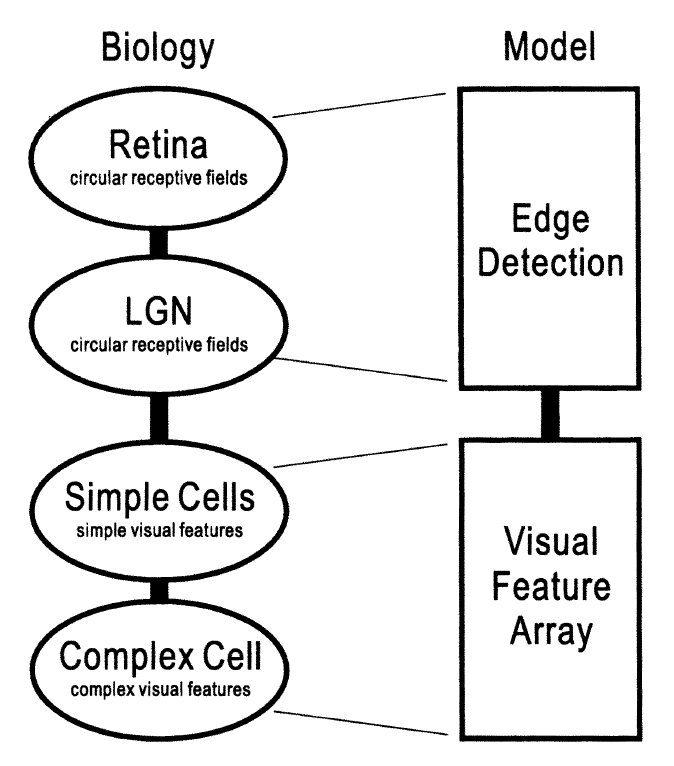
\includegraphics[width=.50\textwidth]{images/vfa_model_idea.png}
%	\caption{Przedstawienie szlaku wzrokowego wraz z pomysłem na model tablicy cech wizualnych \cite{Resko2005}.}
%	\label{fig:vfaIdea}
%\end{figure}

\begin{figure}[ht]
	\centering
	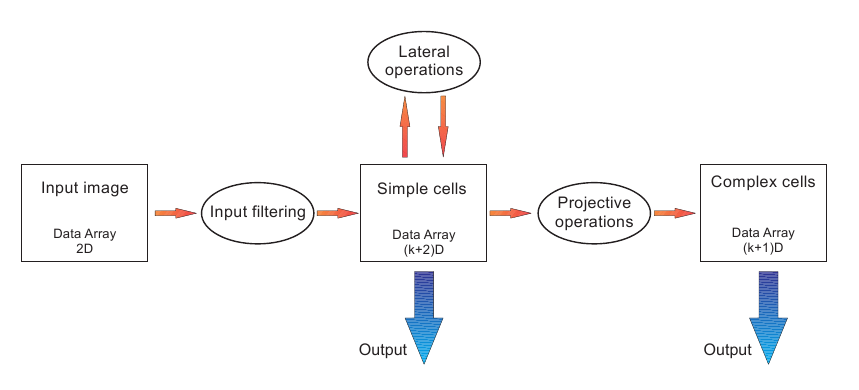
\includegraphics[width=1.00\textwidth]{images/vfa_model.png}
	\caption{Model tablicy cech wizualnych, prostokąty symbolizują struktury danych, elipsy natomiast transformacje \cite{Resko}.}
	\label{fig:vfa}
\end{figure}

\subsubsection{Filtrowanie\\}

Przy tym etapie -- wyodrębniania konturów -- autorzy stosują dosyć dobrze rozpowszechniony w grafice komputerowej filtr Gabora (załącznik \ref{aGabor}). Okazuje się, że natura w korze wzrokowej realizuje coś podobnego do tego matematycznego modelu, co jest opisane dosyć dobrze w pracy \cite{Jones1987}. Świadczy to o tym, że zastosowanie filtru Gabora jest bardzo dobrym krokiem ku celu, którym jest wykorzystanie zalet kory wzrokowej w rozpoznawaniu obrazów.

\subsubsection{Integracja konturów\\}

Na rysunku \ref{fig:vfa} opisana jako ,,Lateral operations''\footnote{Lateral Geniculate Nucleus -- z języka angielskiego -- ciało kolankowate boczne. Jest jednym z elementów szlaku wzrokowego -- którym informacja wizualna jest przenoszona do -- między innymi -- pierwotnej kory wzrokowej, chociaż połączeń jest dużo więcej niż tylko to z pierwszorzędową korą wzrokową. W sensie modelu określenie to ma symbolizować połączenia neuronów sąsiadujących będących w pewnym otoczeniu ze sobą.} integracja konturów, polega na tym, że neurony odpowiedzialne za krawędzie występujące w obrazie pod odpowiednim kątem mają fizyczne połączenie z neuronami odpowiedzialnymi za sąsiednie krawędzie, przez co wpływają na siebie nawzajem.\\

Autorzy założyli, że każda krawędź występująca w obrazie, a otrzymana w momencie ekstrakcji konturów miała przypisaną pewną wartość, która prezentuje jej istotność w obrazie. Wartość ta jest modyfikowana na skutek współdziałania neuronu odpowiedzialnego za tą krawędź z innymi, które z nim sąsiadują. Autorzy uznali, że dobrym podejściem będzie tutaj kombinacja liniowa istotności sąsiednich krawędzi w obrazie.

\subsubsection{Łączenie krawędzi i przedstawienie rezultatów\\}

Mimo, że autorzy dosyć dobrze przedstawili samą teorię potrzebną do realizacji poprzednich etapów, to budowanie cech złożonych -- które jest efektem łączenia krawędzi w większe struktury -- jak i szczegóły dotyczące wcześniejszych etapów jest traktowana po macoszemu -- o czym świadczy brak takich informacji w cytowanych pracach. Można odnieść wrażenie, że przedstawione są tutaj jedynie pomysły, a realizacja jest pozostawiona na uboczu.\\

Otrzymywane wyniki również specjalnie nie zachwycają, ponieważ nietrywialny przykład zastosowania jest tylko jeden, zaczerpnięty z pracy \cite{Resko2005}. 

\begin{figure}[ht]
	\centering
	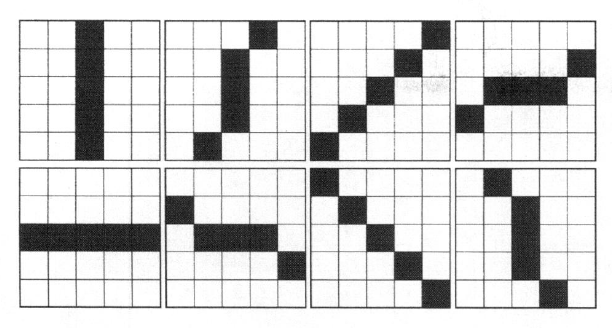
\includegraphics[width=.60\textwidth]{images/vfa_model_neurons.png}
	\caption{Krawędzie z modelu tablicy cech wizualnych, mające reprezentować krawędzie wyodrębnione w obrazie \cite{Resko2005}.}
	\label{fig:vfaModelNeurons}
\end{figure}

\begin{figure}[ht]
	\centering
	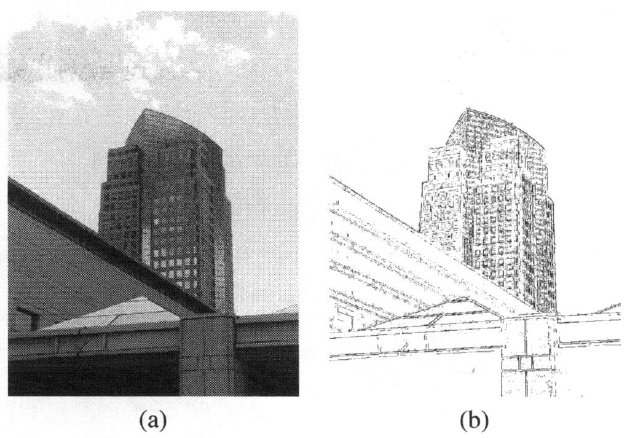
\includegraphics[width=.70\textwidth]{images/vfa_model_results.png}
	\caption{Rezultaty pracy modelu z obrazem: a) obraz wejściowy, b) wyjście z modelu \cite{Resko2005}.}
	\label{fig:vfaModelResults}
\end{figure}


%DONE%TO DO - Hypercolumn - 60k1
\subsection{Hiperkolumna}
\label{hypercolumn}

Patrząc na odzyskiwanie konturów z obrazu różnymi metodami w końcu trafi się na perspektywę, która będzie wywodziła się bezpośrednio z kory wzrokowej. Praca \cite{Curulku} przedstawia szczególny punkt widzenia w kwestii szukania krawędzi w obrazie, można w niej przeczytać o hiperkolumnie, o której wspomniane było w części \ref{v1}. Praca ta mimo, że opisuje tylko pewien model, może przedstawiać dobry pomysł na realizację zadania odzyskiwania konturów w postaci zbliżonej do tych, które są w korze wzrokowej człowieka.\\

\begin{figure}[ht]
	\centering
	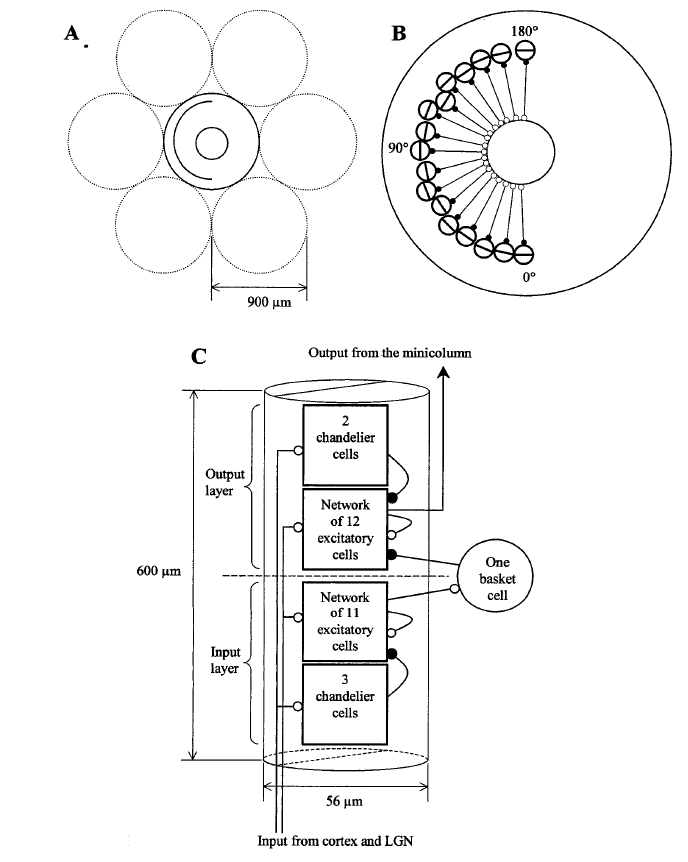
\includegraphics[width=.75\textwidth]{images/Hypercolumn.png}
	\caption{Model hiperkolumny, zaproponowany przez autorów pracy \cite{Curulku}, powstały na podstawie badań kory wzrokowej kota.}
	\label{fig:hypercolumn_model}
\end{figure}

%http://www.informaworld.com/smpp/content~db=all~content=a713663429
%%%Receptors can be classified broadly as excitatory (causing an increase in firing rate), inhibitory (causing a decrease in firing rate), or modulatory (causing long-lasting effects not directly related to firing rate).
Autorzy proponują, aby każdemu obszarowi w obrazie odpowiadała pewna hiperkolumna (rysunek \ref{fig:hypercolumn_model}A) składająca się z 17 różnie ukierunkowanych krawędzi (rysunek \ref{fig:hypercolumn_model}B), które są połączone w ramach tej kolumny w sieć BCPNN\footnote{Bayesian Confidence Propagation Neural Network -- Sieć neuronowa zbudowana na podstawie sieci Bayesowskiej.} mającej za zadanie wybrać spośród 17 krawędzi będących pod różnymi kątami tą najbardziej odpowiednią. Kolumna ta składa się z dwóch warstw (rysunek \ref{fig:hypercolumn_model}C), wejściowej i wyjściowej, w których łącznie 28 neuronów. Nie ma fizycznych połączeń między tymi dwoma warstwami innych niż poprzez jedną komórkę którą autorzy nazwali koszykiem\footnote{Z języka angielskiego -- basket cell.}. Komórka ta pełni rolę inhibitora -- czyli powoduje osłabienie sygnału wyjściowego z neuronów\footnote{W literaturze angielskojęzycznej spotyka się określenie firing rate -- które nie do końca szczęśliwie, ale jest w tej pracy tłumaczone na siłę sygnału wyjściowego. Jest to jednak tylko przeniesienie języka sztucznej inteligencji do stricte biologicznego opisu.}. Połączona jest natomiast z ekscytatorami, czyli komórkami, które powodują wzmocnienie sygnału wyjściowego z neuronów. Wszystkie neurony warstwy wejściowej są połączone z komórką koszykową, przez co mają na nią bezpośredni wpływ. Podobnie z komórkami warstwy wyjściowej, których wejścia sterowane są jedynie z łączącej obie warstwy komórki koszykowej. Dodatkowo w każdej warstwie kolumny znajdują się inhibitory, których zadaniem jest wpływanie na ekscytatory. Widać wyraźnie, że wyjściem z hiperkolumny jest sygnał z ekscytatorów warstwy wyjściowej. Natomiast samo wejście jest przekazywane z ciała kolankowatego bocznego.\\

Opis ten można by kontynuować wprowadzając więcej czysto biologicznych szczegółów. Autor tego dokumentu chciał jednak wprowadzając ten model pokazać z jednej strony, jak interpretowane mogą być odkrycia opisywane w części \ref{v1} tej pracy, z drugiej natomiast przedstawić pewną strukturę, która jest wykorzystywana w kilku kolejnych podejściach stosowanych głównie do symulacji działania pierwszorzędowej kory wzrokowej.




%DONE%TO DO - LI: 37
\subsection{Integracja konturów w pierwszorzędowej korze wzrokowej}
\label{integracjaLi}

%LI - 37
%%%Receptors can be classified broadly as excitatory (causing an increase in firing rate), inhibitory (causing a decrease in firing rate), or modulatory (causing long-lasting effects not directly related to firing rate).

Aby zaczerpnąć z prezentowanych wcześniej technik \ref{integracjaSEC} oraz \ref{hypercolumn} został stworzony inny model ekstrakcji i integracji konturów.\\ 
\begin{figure}[ht]
	\centering
	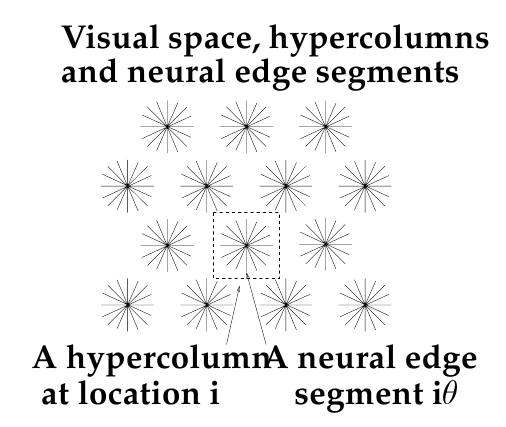
\includegraphics[width=0.55\textwidth]{images/li_hypercolumn.png}
	\caption{Przestrzeń hiperkolumn w modelu integracji konturów \cite{Li1998}.}
	\label{fig:li_hypercolumn}
\end{figure}

\begin{figure}[ht]
	\centering
	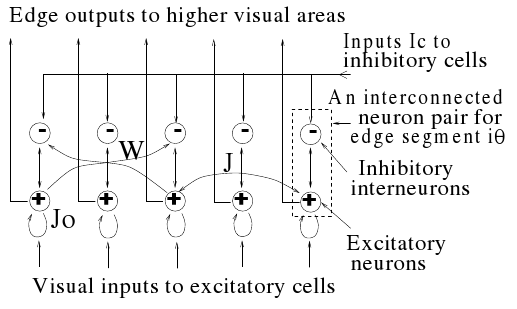
\includegraphics[width=0.7\textwidth]{images/li_arch.png}
	\caption{Architektura częściowa sieci prezentującej podstawowe elementy składowe modelu z pracy \cite{Li1998}.}
	\label{fig:li_arch}
\end{figure}

Podstawowym elementem modelu integracji konturów jest hiperkolumna -- która zgodnie z tym co zostało zaobserwowane w korze wzrokowej kota -- jest ona umieszczona w heksagonalnej przestrzeni, co znaczy, że każda z nich 6 sąsiadujących. Składa się ona z segmentów krawędziowych\footnote{Tłumaczenie z języka angielskiego -- edge segment.}, a każdy segment może zostać określony numerem kolumny $i$ w przypadku jeśli wszystkie są ponumerowane oraz kątem $\theta$ który odpowiada za nachylenie krawędzi w segmencie. W każdym segmencie znajduje się para neuronów, inhibitor i ekscytator, które są ze sobą połączone. Gdy w części obrazu objętej obszarem $i$ znajduje się krawędź zorientowana pod kątem $\beta$ oraz siłą/intensywnością $\hat{I}_{i\beta}$ (rysunek \ref{fig:li_hypercolumn}), wtedy segment otrzymuje na wejście sygnał $I_{i\beta}$ który można wyliczyć z poniższego wzoru. 
$$I_{i\beta} = \hat{I}_{i\beta} \phi (\theta - \beta)$$ 
gdzie 
$$\phi(\theta - \beta) = e^{-|\theta - \beta| / (\phi / 8 )}$$
jest pewną funkcją odchylenia. Rzecz jasna segmenty poza hiperkolumną nie dostają żadnego sygnału.\\
Określa się też parametr nazywany barierą membranową oznaczaną $x_{i\theta}$ dla ekscytatora oraz $y_{i\theta}$ dla inhibitora oraz funkcje wyjścia dla każdego z neuronów $g_x(x_{i\theta})$ oraz $g_y(y_{i\theta})$.\\
Architektura tej sieci jest zaprezentowana na rysunku \ref{fig:li_arch}.\\

\begin{figure}[ht]
	\centering
	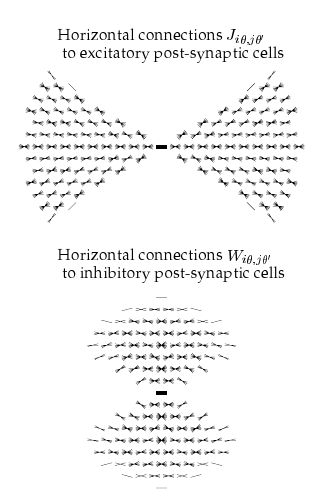
\includegraphics[width=0.45\textwidth]{images/li_field.png}
	\caption{Pole mające wpływ na konkretny jeden segment, w zależności od funkcji odległości $J_{i\theta, j\theta'}$ oraz $W_{i\theta, j\theta'}$ \cite{Li1998}.}
	\label{fig:li_rf}
\end{figure}

Wyniki działania modelu -- wprawdzie skąpe, są przedstawione na rysunku \ref{fig:li_out}.\\

\begin{figure}[ht]
	\centering
	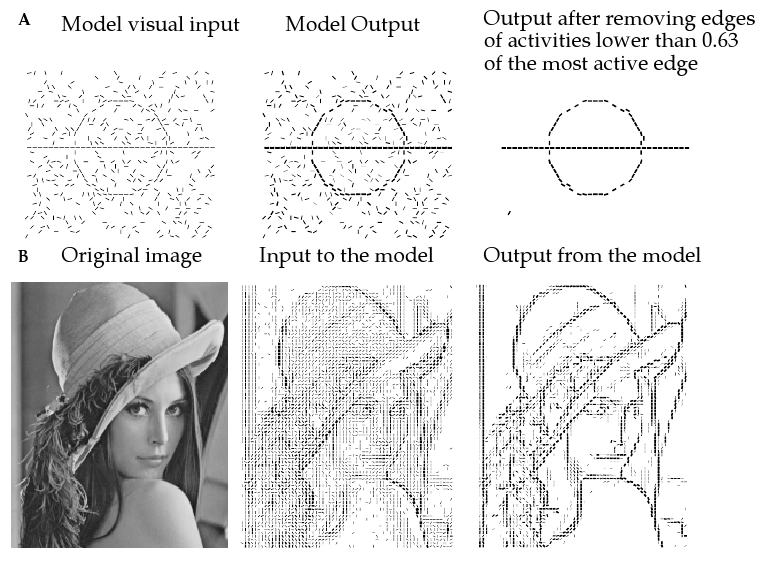
\includegraphics[width=1.00\textwidth]{images/li_out.png}
	\caption{Wyniki działania opisanego wcześniej algorytmu. Praca przedstawia zdjęcie najczęściej poddawane obróbce cyfrowej -- Lenę. Wyraźnie widać, że krawędzie zostały odzyskane w praktycznie doskonały sposób \cite{Li1998}.}
	\label{fig:li_out}
\end{figure}

Autor cytowanej pracy zwraca uwagę na połączenia między-segmentowe. Wyraźnie widać je na schemacie prezentującym architekturę sieci. Co jest istotne, są one realizowane jedynie na 2 sposoby: między ekscytatorami różnych segmentów oraz między ekscytatorem i inhibitorem z różnych segmentów. Nie ma połączeń między inhibitorami, nawet na siebie.\\

Sens sieci jest taki, aby ona się omiatała przez jakiś czas i ustalała swój stan. Konieczne jest bowiem propagowanie wyników -- sygnałów wyjściowych po raz kolejny do wejść neuronów oraz przeliczanie od nowa. Bardzo dobrze jest to przedstawione na rysunku \ref{fig:li_arch}.\\
Aby jednak móc lepiej zaprezentować działanie całości potrzeba trochę formalizmów, których w pracy \cite{Li1998} nie brakuje. 
\begin{align}\label{eqn:li_wzor1}
\dot{x}_{i\theta} = - \alpha_xx_{i\theta} - \sum_{\Delta\theta}\psi(\Delta\theta)g_y(y_{i\theta+\Delta\theta})+ \notag\\
+ J_0g_x(x_{i\theta}) + \sum_{j \neq i, \theta'} J_{i\theta, j\theta'}g_x(x_{j\theta'}) + I_{i\theta} + I_0
\end{align}
\begin{align}\label{eqn:li_wzor2}
\dot{y}_{i\theta} = - \alpha_yy_{i\theta} - g_x(x_{i\theta}) + \sum_{j \neq i, \theta'} W_{i\theta, j\theta'}g_x(x_{j\theta'}) + I_c
\end{align}
Wzory \ref{eqn:li_wzor1} oraz \ref{eqn:li_wzor2} prezentują wyjściowe stany w tak zwanym momencie '$t+1$'. Występujące we wzorach $J_{i\theta, j\theta'}$ oraz $W_{i\theta, j\theta'}$ są w pewnym sensie funkcjami odległości $j\theta'$ od $i\theta$. Funkcje te są pewnej nieprzystępnej postaci -- wyznaczonej doświadczalnie i nie będą tutaj umieszczane, konieczne jest jednak pokazanie sensu tych funkcji. Można go zaprezentować określając pole, jakie ma znaczenie biorąc pod uwagę wpływ sąsiednich pól, na jedno -- konkretne. Przedstawione ono jest na rysunku \ref{fig:li_rf}.\\


Omawiając to podejście należy wspomnieć o uwagach autorki publikacji \cite{Li1998} z której zostały zaczerpnięte przykłady. We wstępie swojej pracy zwraca Ona uwagę na problematykę etapu ekstrakcji konturów z obrazu. Wymienia kilka różnych algorytmów, na które mają związek z tym, jak kontury odzyskiwane są w korze wzrokowej. Zwraca uwagę jednak na to, że nawet bez ograniczeń wynikających z zastosowania podejścia wzorowanego na pierwszorzędowej korze wzrokowej jest to zagadnienie trudne. Wspominany w części \ref{integracjaSEC} algorytm na proste i skuteczne odzyskiwanie krawędzi z obrazu, wprawdzie nie był zastosowany w opisywanej pracy, ale inne algorytmy tego pokroju były przez autorkę testowane. Odnosi się bowiem Ona do nich jako do algorytmów mających problem. Najczęściej wynika on z występowania parametrów, które wymagają dostrojenia przez użytkownika, przez co do dobrej symulacji ekstrakcji konturów nie mogą być zastosowane.\\

Autorka stawia nawet pytanie, czy jest to osiągalne za pomocą modelowania obszaru V1 mózgu, czy może to wymagać wpływu wyższych warstw kory wzrokowej. Opisywane wcześniej biologiczne podstawy funkcjonowania kory wzrokowej wskazują, że może to być bardzo prawdopodobne.


%DONE%TO DO - SPIKE: 90k4
\subsection{Integracja konturów modelem integrate-and-fire}
\label{integracjaSPIKE}

\begin{figure}[ht]
	\centering
	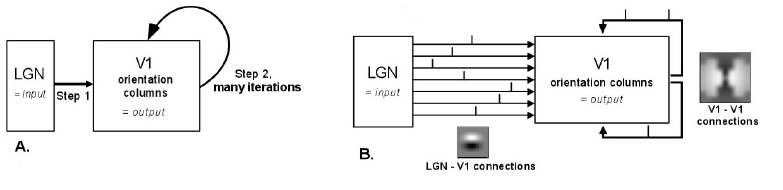
\includegraphics[width=1\textwidth]{images/spike_model.png}
	\caption{Przedstawienie porównań modeli integracji konturów w pierwszorzędowej korze wzrokowej \cite{Vanrullen2001}.}
	\label{fig:spike_model}
\end{figure}

%\begin{figure}[ht]
%	\centering
%	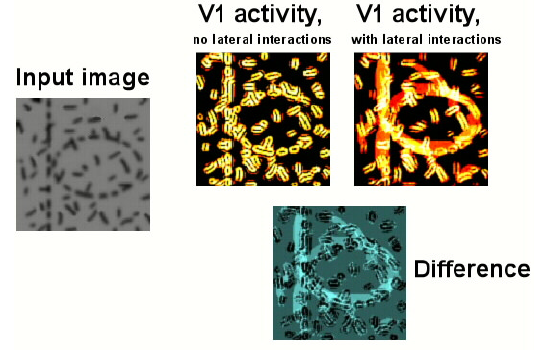
\includegraphics[width=0.65\textwidth]{images/spike_model_out_1.png}
%	\caption{ \cite{Vanrullen2001}.}
%	\label{fig:spike_model_out_1}
%\end{figure}

%\begin{figure}[ht]
%	\centering
%	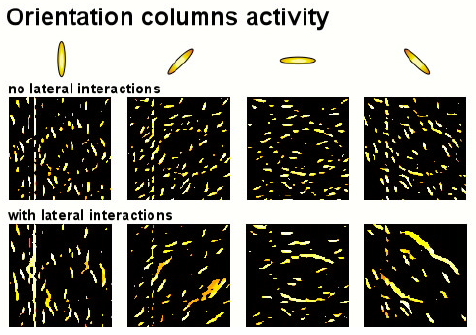
\includegraphics[width=0.65\textwidth]{images/spike_model_out_2.png}
%	\caption{ \cite{Vanrullen2001}.}
%	\label{fig:spike_model_out_2}
%\end{figure}

\begin{figure}[ht]
	\centering
	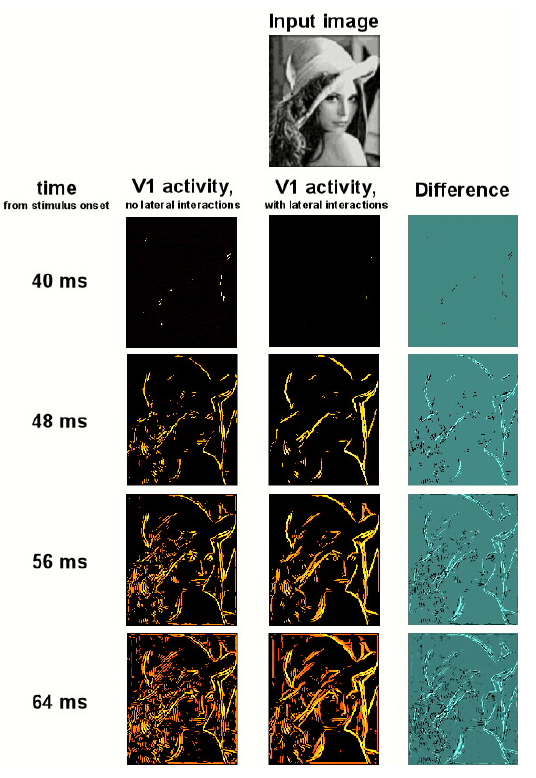
\includegraphics[width=0.65\textwidth]{images/spike_model_results.png}
	\caption{Porównanie wyników otrzymywanych z modelu ,,integrate-and-fire'' ze sprzężeniem i bez \cite{Vanrullen2001}.}
	\label{fig:spike_model_results}
\end{figure}
%spike - 10003
%TODO - przeformułowanie początku

Autorzy pracy \cite{Vanrullen2001} zauważyli pewien mankament zwłaszcza wydajnościowy w modelu przedstawionym choćby w poprzedniej części -- \ref{integracjaLi}. Podstawową jego cechą były dziesiątki połączeń miedzy neuronami z hiperkolumn, przez co przeliczanie się całości trwało jakiś czas. Na podobnej zasadzie autorzy przytaczają też inne publikacje.\\

Głównym argumentem -- który zdaniem autora tego dokumentu jest śmieszny -- który stał za wnioskiem, że wyliczone modele są złe, był czas ich działania. Porównując je bowiem z błyskawicznym\footnote{W publikacji jest to określone angielskim słowem rapid.} przetwarzaniem obrazów w korze wzrokowej człowieka, bądź małpy, muszą one być w sprzeczności z całą biologią, która za tym stoi. Nie podejmowano jednak argumentu, że w mózgu absolutnie wszystko jest ,,przeliczane'' równolegle i nie ma w nim miejsca na iteracje znane z komputerowych implementacji sieci neuronowych. Nie mniej jednak proponuje się w tej pracy specyficzne podejście bazujące na modelu ,,sumuj i strzelaj\footnote{Tłumaczenie z języka angielskiego frazy integrate-and-fire, którą można nazwać inaczej modelem Lapicque'a\cite{Lapicque}.}''. Zaproponowany model przedstawia rysunek \ref{fig:spike_model}B. Autorzy porównują go do proponowanych w innych pracach iteracyjnych podejść, które przedstawione są na rysunku \ref{fig:spike_model}A. Na pierwszy rzut oka nie widać specjalnie różnic, podstawowa wynikająca z zastosowania podejścia Lapicque'a jest jednak -- zdaniem autorów -- kluczowa.\\

W modelu widać wyraźnie sprzężenie zwrotne i mimo, że są one krytykowane w cytowanych wcześniej pracach, to autorzy podkreślają, że to nie jest problem samych sprzężeń. Chodzi, raczej o to, że w klasycznych modelach sprzężenie zwrotne działa po przeliczeniu się wszystkich neuronów, tutaj jednak, przez wzgląd na obserwacje kory wzrokowej kota sprzężenie zwrotne cały czas ma wpływ na neurony warstwy V1. Całą implementację upraszcza dodatkowo fakt, że przez połączenia prowadzone są jedynie pewne piki, a same neurony zliczają je i na tej podstawie określają swój stan. Nie potrzeba tutaj przesyłania ciągłych sygnałów.\\

Rysunek \ref{fig:spike_model_results} przedstawia otrzymywane w ten sposób rezultaty, które zgodnie z poprzednim akapitem zostały sobie przeciwstawione. Po lewej stronie rezultaty prezentują wyjście z modelu, w którym połączeń między elementami pierwszorzędowej kory wzrokowej nie ma, środkowe obrazy przedstawiają te same wyniki modelu, z różnicą na występowanie połączeń między elementami V1. Prawa kolumna pokazuje różnice między opisanymi rezultatami. Tak jak i w dziesiątkach książek poświęconych grafice komputerowej i tutaj obrazem do testowania była Lena. Podstawowym parametrem modelu jest czas, jaki się poświęca przeliczeniom samego modelu. Otrzymywane rezultaty przedstawiają przede wszystkim zalety korzystania z połączeń między elementami obszaru V1 jak i samego pomysłu na realizację integracji konturów w korze wzrokowej.\\



%DONE%TO DO - GPC: 50k5
\subsection{@@@@integracja GPC}
\label{integracjaGPC}

%gpc - 50k5


%TO DO - RV1: 20k11
%\subsection{@@@@integracja RV1}
\label{integracjaRV1}

%RV1 - 20k11

%% słaba jakość modelu, dużo opisu głupot i wyprowadzania śmiesznych przekształceń, a wyniki też mizernie zaprezentowane.

%%
%40k16
%%

%TO DO - CDCI - , 40k19, 
%\subsection{@@@@integracja CDCI}
\label{integracjaCDCI}

%cdci - 40k16
% - 40k19

%%% to nie są pojedyncze krawędzie, ani integracja...

%TO DO - active contours?? - 40k21, 30k6
%%%\subsection{@@@@integracja AC}
\label{integracjaAC}

%AC - 40k21
% - 30k6

%%%brak kory wzrokowej....

%TO DO - POGGIO: 63, 64, 1, 3, 73, ~20k12, 16, 39
%TO DO @UP modif - 41
\subsection{@@@@integracja POGGIO}
\label{integracjaPOGGIO}

%TODO - POGGIO: 63, 64, 1, 3, 73, ~20k12, 16, 39
%TODO @UP modif - 41


%TO DO - posprawdzać ToDosy, 
%TO DO - opisać przyszłość, 
%TODO - trudności (invariant), 
%TO DO - może ontologia?

\section{Podsumowanie}
\label{Chapter1_sumUp}

W dalszej części tej pracy przedstawiony będzie szczegółowy opis proponowanego przez autora podejścia, które w dużej mierze czerpać będzie z przedstawionych w literaturze modeli mory wzrokowej człowieka. Wstępnie można by nakreślić kroki, jakimi warto by było zrealizować cel postawiony w temacie tej pracy. 

\newcounter{Lcount}
\begin{list}{\textbf{\Roman{Lcount}}}
    {\usecounter{Lcount}
    \setlength{\rightmargin}{\leftmargin}}\label{proponowane_etapy_realizacji_pracy}
\item \textbf{Odzyskiwanie krawędzi z obrazów} -- czyli zastosowanie filtrów Gabora do wyszczególnienia krawędzi w zadanych obrazach. \\
Zawartość załącznika \ref{aGabor} świadczy o realizacji tego etapu.
\item \textbf{Ekstrakcja krawędzi z przefiltrowanych obrazów} -- wydobycie krawędzi czyli pewnych kresek -- mających reprezentować krawędzie obiektów występujących w niewielkich fragmentach obrazu. \\
Nawiązując do wcześniejszych części tej pracy -- jest to etap trudny i przy realizacji pod uwagę będzie branych wiele różnych algorytmów, wstępnie jednak nieokreślonych.
\item \textbf{Integracja konturów} -- pozostawienie w obrazie przedstawionym za pomocą krawędzi jedynie tych, które są istotne ze względu na to, że są częścią złożonej krawędzi, a nie zakłóceniem.\\
Wstępnie można by założyć wykorzystanie jednego z opisanych wcześniej podejść \ref{integracjaLi}, \ref{integracjaSPIKE} lub \ref{integracjaGPC}, ale autor wstępnie nie chce się przywiązywać specjalnie do konkretnego rozwiązania.
\item \textbf{Budowanie cech złożonych} -- składanie krawędzi z poprzedniego etapu w większe struktury.\\
Podobnie jak to jest zaproponowane w części \ref{integracjaPOGGIO}, liczba -- wprawdzie nie cytowanych, ale istniejących -- prac wskazuje na to, że hierarchiczne podejście jest dobrym rozwiązaniem.
\item \textbf{Podział na obiekty występujące w obrazie} -- podział stworzonych w poprzednim etapie szkieletów -- reprezentujących odnalezione w obrazie krawędzie -- na obiekty ze względu na różnicę w kolorach.\\
Coś, co wydaje się być oczywiste. Przegląd literatury jednak nie wskazuje, żeby było to popularne rozwiązanie.
\item \textbf{Klasyfikacja wydzielonych obiektów} -- przypisanie odnalezionemu obiektowi jego klasy -- nazwanie obiektu z obrazu.\\
W niektórych pracach jest ten etap rozwiązywany jako sieć neuronowa -- która z definicji jest klasyfikatorem. Autor rozważa zastosowanie w tym etapie sieci neuronowej, natomiast planuje również zbudowanie ontologii z klas, do których będą należeć obrazy dla stworzonego modelu. Konieczne jest również zebranie odpowiedniej liczby samych obrazów, na których model będzie pracował, ucząc się i szukając podobnych -- czyli -- realizując temat. Konieczna jest dodatkowo różnorodność obrazów, aby ontologia mogła prezentować pewną hierarchię.
\end{list}

Autor planuje realizację tych etapów we właśnie takiej kolejności jak na liście powyżej, z zastrzeżeniem jednak, że zbieranie obrazów oraz budowanie ontologii z ostatniego etapu, ponieważ nie zależy od żadnego z nich, może być przeprowadzone równolegle z dowolnym.


%%
%%TO DO - object perception
%%
% 00018 - object perception....

%%
%Proposed: 20k7, 30k8, 40k20, 30k7, 50k3, 90k7, 30k31
%TO DO - Snake: 30k16, 30k24, 30k29, 30k32
%TO DO - 30k14- overview
%%


%TO DO - BAYES: 2,

%TO DO - propozycja własnego podejścia - opis użytych już podejść itd...
%\subsection{Ekstrakcja konturów z obrazu}
\label{integracjaSEC}

%SEC - 30k10
%http://www.int.washington.edu/talks/WorkShops/int_03_1/People/Schlei_B/INT2003.pdf

Algorytmów na ekstrakcję konturów z obrazu jest bardzo wiele, na dziesiątki różnych sposobów można szukać krawędzi obiektów na nich się znajdujących. Mimo, że jest ich wiele, i wyniki ich działania są zadowalające -- chociaż z entuzjazmem najczęściej wypowiadają się sami autorzy -- to problem jest trochę gdzie indziej. Krawędzie odzyskane z obrazów klasycznymi algorytmami, wciąż są pikslami w obrazie, które wprawdzie dla ludzkiego oka stanowią lepsze lub gorsze odwzorowanie konturów, ale do dalszego przetwarzania muszą być dodatkowo przygotowane. Jest to spowodowane przede wszystkim wymaganiami podyktowanymi przez temat tej pracy, który zakłada czerpanie z kory wzrokowej jako źródła inspiracji dla algorytmów. W związku z czym wymagane jest przetwarzanie otrzymanych obrazów przedstawiających krawędzie do struktur danych reprezentujących te krawędzie.\\

Przedstawiony więc będzie jeden z wielu algorytmów, który z obrazów odzyskuje kontury z obrazu cyfrowego.


\label{diconex}
\subsubsection{DICONEX}

Algorytm -- co podkreślają twórcy -- jest perfekcyjny w sensie wyznaczania krawędzi obiektów jeśli przyjmie się następujące kryteria:
\begin{itemize}
\item obszary się wzajemnie nie przecinają,
\item obszary są niepuste,
\item nie ma ograniczeń na 2 wymiary,
\item szybkość działania
\end{itemize}
Algorytm pracuje na obrazach monochromatycznych, więc wymaga się przekształcenia np. zdjęć do skali szarości.

\begin{figure}[ht]
	\centering
	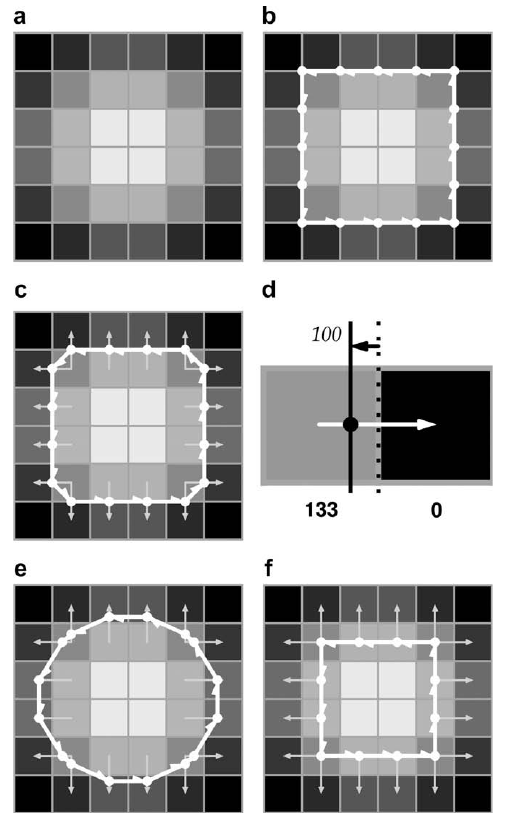
\includegraphics[width=.55\textwidth]{images/DICONEX_EX.png}
	\caption{Przykład działania algorytmu DICONEX na obrazie w skali szarości, o rozmiarach $6 \times 6$ \cite{Schlei2009}.}
	\label{fig:diconex_ex}
\end{figure}

\begin{figure}[ht]
	\centering
	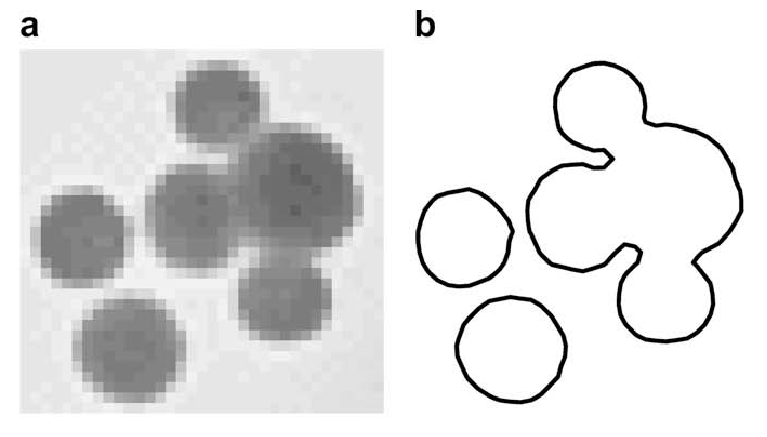
\includegraphics[width=.70\textwidth]{images/DICONEX_EX_RES.png}
	\caption{Wynik (b) działania algorytmu DICONEX na obrazie niewielkiej rozdzielczości (a) \cite{Schlei2009}.}
	\label{fig:diconex_ex_res}
\end{figure}

\label{dixonex_alg}
\subsubsection{Algorytm}

Na początku algorytmu wymagane jest wybranie jednej -- granicznej wartości jasności dla obrazu. W przykładzie z pracy \cite{Schlei2009}, dla obrazu, którego jasność piksli jest z zakresu $0 - 155$ została ona obrana na poziomie 100. Rysunek \ref{fig:diconex_ex}A przedstawia wejściowy obraz. W pierwszym kroku algorytmu, w obrazie wektorami konturowymi (ang. contour vector) otaczane są piksle o wartości jasności większej niż 100 -- czyli jasne piksle -- czego wynik przedstawiany jest na rysunku \ref{fig:diconex_ex}b. Warto zauważyć, że wspomniane wektory konturowe zawsze zwrócone są w taką stronę, że po lewej stronie mają otaczany obiekt -- czyli w tym wypadku piksle o jasności większej niż 100. Zgodnie z tym algorytmem zawsze znalezione wektory będą ze sobą połączone na zasadzie początek jednego wektora z końcem drugiego wektora i nie będzie pustych obszarów. Jako kolejny krok algorytmu, wszystkie stworzone wektory zamieniane są na inne wektory, o tej samej orientacji, ale ich punkty zaczepienia znajdują się w na środku wyznaczonego wcześniej wektora krawędziowego (konturowego), a kończą się w środku kolejnego wektora krawędziowego. Po zastosowaniu się do tego przekształcenia obraz otrzymany powinien wraz z krawędzią wyglądać tak jak na rysunku \ref{fig:diconex_ex}c. Dodatkowo na tym rysunku przedstawione są pewne wektory, które w cytowanej publikacji nazywane są wektorami zakresu (ang. range vector). Wektory te są umieszczone w obrazie w taki sposób, że łączą środki sąsiednich piksli i przechodzą przez każdy środek wektora konturowego a ich zwrot jest skierowany na zewnątrz otaczanego obszaru. Rysunek \ref{fig:diconex_ex}d przedstawia 2 piksle z obrazu, między którymi znajdował się środek wektora konturowego. W kolejnym kroku algorytmu punkt ten będzie przesunięty na wektorze zakresu w taki sposób, że obrana na samym początku wartość jasności (równa 100) będzie znajdować się na tym wektorze, gdy między środkowymi punktami piksli wartość ich jasności będzie liniowo interpolowana. Wynik takiego działania przedstawiony jest na rysunku \ref{fig:diconex_ex}e. Rysunek \ref{fig:diconex_ex}f przedstawia wynik transformacji tego poszerzonego konturu do konturu oznaczającego granicę szukanego obszaru. Jednak jak widać na przykładzie to przekształcenie jakby cofało wszystkie uogólnienia, zaokrąglenia i właściwie same przekształcenia, które zostały znalezione w obrazie \ref{fig:diconex_ex}c i \ref{fig:diconex_ex}e. Zdaniem autora najlepszy rezultat zaprezentowany jest na rysunku \ref{fig:diconex_ex}e.\\

O ile sam algorytm jest ciekawy, to został on tutaj zaprezentowany głównie z powodu na efekty, jakie można uzyskać w innych nietrywialnych obrazach, w a szczególności tych, niewielkich rozmiarów. Rysunek \ref{fig:diconex_ex_res} przedstawia wynik działania algorytmu na obrazie słabej rozdzielczości. Wyraźnie widać, że kontury odtworzone przez algorytm są wyraźne i gładkie, co jest niewątpliwą zaletą.\\

Z zastosowaniem tego algorytmu jest jednak podstawowy problem, który polega na konieczności obrania wartości granicznej dla jasności grup piksli w obrazie. Podobne problemy mają inne algorytmy odnajdujące krawędzie w obrazie. Można by się spierać, który jest lepszy, fakt jest jednak taki, że w oryginalnej postaci wymagają określania dodatkowych specyficznych parametrów.\\

Trochę inaczej można podejść do tego zagadnienia metodami zaczerpniętymi wprost z grafiki komputerowej -- filtrami. Dla obrazów binarnych (dwukolorowych) bardzo prosto jest określić okno filtru, który miałby odzyskać same krawędzie z obszarów przedstawionych w obrazie \cite{Tadeusiewicz}. Dla obrazów w skali szarości można posłużyć się bardziej zaawansowanymi filtrami, w tym na przykład filtrem Gabora, o którym dokładniej w części \ref{aGabor}.



 - jako proponowane... no i że jest wiele innych możliwości.




\appendix

\chapter{Filtr Gabora}
\label{aGabor}
%TODO S pending!
\section{Teoria}
\label{aGabor_teoria}
Filtr w grafice komputerowej jest tak zwaną konwolucją dyskretną \cite{Tadeusiewicz} obrazu. Dla przypadku 2 wymiarów będzie ona przedstawiona poniżej.
$$
	L'(m, n) = (w \times L)(m, n) = \sum_{i, j \in K}L(m-i, n-j)w(i, j)	
$$
Należy wyjaśnić, że w powyższym przykładzie $L$ jest obrazem początkowym, gdzie $L(x, y)$ jest punktem w tym obrazie określonym współrzędnymi $x$ i $y$. Natomiast $w(x, y)$ jest filtrem, którego składowe $x$ i $y$ są tak samo interpretowane. Wynikiem przedstawionej w ten sposób filtracji obrazu jest $L'$.\\
Można powiedzieć, że przy filtrowaniu posiadamy 3 macierze/tablice(2D) różnych rozmiarów. Z czego przyjmuje się, że macierze $L$ i $L'$ są tych samych rozmiarów, a macierz $w$ jest innych rozmiarów (najlepiej aby jej rozmiary przedstawiane były za pomocą 2 liczb nieparzystych) i jest dużo mniejsza od $L$. Macierz $w$ jest 'oknem filtru'.\\

Filtrowanie jest procesem w którym dla każdego piksela z obrazu wejściowego -- nawiązując do oznaczeń zaproponowanych powyżej -- $L$ kolor odpowiadającego mu piksla w obrazie wyjściowym ($L'$) jest zależny od ważonej sumy wartości koloru piksli go otaczających. Wagi dla tego przekształcenia są określone przez okno filtru i przyjmuje się, że środkowemu punktowi okna filtru odpowiada wybrany wcześniej piksel w obrazie $L$. Dodatkowo wymaga się, aby zostały określone warunki na podstawie których będzie można to przekształcenie stosować na krawędziach obrazu, dochodzi tam bowiem do sytuacji, w których okno filtru wykracza poza obraz. Przyjmuje się, że w takich wypadkach nieistniejące piksle nie biorą udziału w wyliczeniach wartości koloru dla danego piksla leżącego przy krawędzi. Należy jednak dodatkowo zwrócić uwagę na fakt, że obraz jest dwuwymiarową tablicą kolorów, z których każdy jest w określonych granicach. Wymagane jest więc, aby po przekształceniu obrazu danym filtrem doprowadzić jego wartości kolorów w taki sposób, aby mógł on odzwierciedlać obraz.\\

Przykładowo obraz może być dwuwymiarową tablicą piksli, z których każdy jest określonego koloru, a kolor ten jest przedstawiony np. jako wartość jasności (dla obrazów czarno-białych) i mieści się w zakresie $(0, 255)$. Po przekształceniu filtrem o oknie wielkości $3\times3$, w którym wartości są z zakresu $(-1, 1)$ należałoby wartości w obrazie wynikowym tak przemnożyć, aby również przedstawiały określony wcześniej zakres. 

\subsection{Funkcja Gabora}
\label{aGabor_funkcja}

Funkcja Gabora \cite{Movellan}, która jest głównym składnikiem filtru Gabora jest bardzo prostym złożeniem dwóch, tak naprawdę elementarnych funkcji. Jako złożenie funkcji autor ma na myśli prosty iloczyn -- jak to jest przedstawione we wzorze \ref{eqn:aGabor_wzor1}.
\begin{align}\label{eqn:aGabor_wzor1}
g(x, y) = s(x, y) w_r (x, y)
\end{align}
W przedstawionym powyżej wzorze należy wyszczególnić dwa elementy: 
\begin{description}
\item [$s(x, y)$] -- jest zespoloną sinusoidą, nazywaną nośnikiem\footnote{Z języka angielskiego carrier.}
\item [$w_r (x, y)$] -- jest dwuwymiarową funkcją o kształcie funkcji Gaussa, nazywaną powłoką\footnote{Z języka angielskiego envelope.}
\end{description}

\subsubsection{Nośnik}
\label{aGabor_carrier}

Zespolona sinusoida jest odwzorowaniem funkcji \ref{eqn:aGabor_c_sinus} na płaszczyźnie.
\begin{align}\label{eqn:aGabor_c_sinus}
s(x, y) = exp(j(2\pi(u_0x + v_0y)+P))
\end{align}
W podanym wyżej wzorze można wydzielić parametry:
\begin{description}
\item [$P$] -- faza sinusoidy
\item [$(u_0, v_0)$] -- wektor, który opisuje częstotliwość sinusoidy
\end{description}

\subsubsection{Powłoka}
\label{aGabor_envelope}

\subsection{Filtr Gabora}
\label{aGabor_filtr}

%TODO - screeny i uszczegółowienie

\subsection{Przykład filtrowania}
\label{aGabor_przyklad}

%TODO no jak sama nazwa wskazuje - przykłady

\section{Dyskusja i wnioski}
\label{aGabor_dyskusja}

%TODO - trochę o tym, że to dobre!



\pagestyle{plain}
 
\listoffigures
\listoftables
\listofalgorithms

\bibliographystyle{iisthesis}
\bibliography{MAS}
\end{document}

